\chapter{解析几何}

在第 2 章中,我们在一般但抽象的层次上研究了向量、向量空间和线性映射。
在本章中,我们将为所有这些概念增加一些几何解释和直觉感受。
特别是,我们将研究几何向量并计算它们的长度和两个向量之间的距离以及角度。
为了能够做到这一点,我们为向量空间装备了内积,该内积会引出向量空间的几何概念。
内积及其相应的范数度量了相似性和距离这样的直觉概念,
我们在第 12 章中使用它们来开发支持向量机(support vector machine)。
然后我们将使用向量的长度和向量间角度的概念来讨论正交投影,
当我们在第 10 章讨论主成分分析和在第 9 章通过最大似然估计进行回归时,
它是一个核心角色。
图 3.1 概述了本章中的概念如何联系以及它们如何与本书的其他章节联系起来。

\begin{figure}[H]
\begin{tikzpicture}[-latex,rounded corners,xscale=1.3]
        \node[fill=blue!20] (Inner_product) at (3,7) {内积};
        \node[fill=blue!20] (Norm) at (0,5) {范数};
        \node[fill=blue!20] (Lengths) at (0,3) {长度};
        \node[fill=blue!20] (Orthogonal_projection) at (3,3) {正交投影};
        \node[fill=blue!20] (Angles) at (6,3) {(夹)角};
        \node[fill=blue!20] (Rotations) at (9,3) {旋转};
        \node[fill=green!20] (chp4) at (4,0) {Chapter4\\矩阵分解};
        \node[fill=green!20] (chp9) at (0,0) {Chapter9\\回归};
        \node[fill=green!20] (chp10) at (9,0) {Chapter10\\降维};
        \node[fill=green!20] (chp12) at (9,5) {Chapter12\\分类};
        \draw[dashed] (Inner_product) --node[above,rotate=30]{导出} (Norm);
        \draw (Inner_product) -- (Orthogonal_projection);
        \draw (Inner_product) -- (Angles);
        \draw (Inner_product) -- (Rotations);
        \draw (Inner_product) -- (chp12);
        \draw (Norm) -- (Lengths);
        \draw (Norm) -- (Orthogonal_projection);
        \draw (Lengths) -- (chp9);
        \draw (Lengths) -- (chp4);
        \draw (Lengths) -- (Orthogonal_projection);
        \draw (Orthogonal_projection) -- (chp9);
        \draw (Orthogonal_projection) -- (chp10);
        \draw (Orthogonal_projection) -- (chp12);
        \draw (Angles) -- (chp12);
        \draw (Angles) -- (chp4);
        \draw (Angles) -- (Orthogonal_projection);
        \draw (Angles) -- (Rotations);
        \draw (Angles) -- (Rotations);
        \draw (Rotations) -- (chp4);
        \draw (Rotations) -- (chp10);
    \end{tikzpicture}
    \caption{本章概念的思维导图, 以及在其他章节的使用情况}
\end{figure}

\section{范数}
当我们想到几何向量,即从原点开始的有向线段时,
直观上向量的长度就是这条有向线段的“末端”到原点的距离。
下面,我们将使用范数记号讨论向量长度的概念。

\begin{definition}[范数]
    向量空间$V$上的范数(norm)是一个函数
    \begin{align}
        \| \cdot \| : V &\rightarrow \R,\\
        \x &\mapsto \|\x\|,
    \end{align}
    它为每个向量$\x$分配其长度$\|\x\| \in \R$,
    这样对于所有$\lambda \in \R$和$\x, \y \in V$,以下成立:
    \begin{itemize}
        \item 绝对齐次(absolutely homogeneous): $\|\lambda\x\| = |\lambda|\|\x\|$
        \item 三角不等式(triangle inequality): $\|\x+\y\| \leqslant \|\x\| + \|\y\|$
        \item 正定(positive definite): $\|\x\| \geqslant 0$且$\|\x\| = 0 \Longleftrightarrow \x = \0$
    \end{itemize}
\end{definition}

在几何学上,三角不等式指出,对于任何三角形,任意两条边的长度之和必须大于或等于第三边的长度;参见图 3.2 的说明。
定义 3.1 是根据一般向量空间$V$(第 2.4 节)的,但在本书中,我们将只考虑有限维向量空间$\R^n$。
回想一下,对于向量$\x \in \R^n$,我们使用下标表示向量的元素,
即$x_i$是向量$\x$的第$i$个元素。

\begin{figure}[H]
    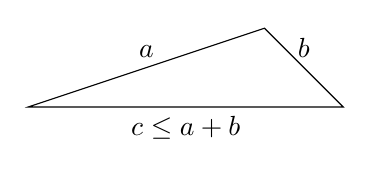
\begin{tikzpicture}
        \draw (0,0)
              -- node[above]{$a$} (3,1)
              -- node[above]{$b$} (4,0)
              -- node[below]{$c \le a + b$} cycle;
    \end{tikzpicture}
    \caption{三角不等式}
\end{figure}

\begin{example}[曼哈顿范数]
    $\R^n$上的曼哈顿范数(Manhattan Norm)被定义为, 对于$\x \in \R^n$
    \begin{equation}
        \|\x\|_1 := \sum^n_{i=1}|x_i|,
    \end{equation}
    其中$|\cdot|$是绝对值.
    图3.3的左图显示了$\|\x\|_1 = 1$的所有向量$\x \in \R^2$.
    曼哈顿范数也称作$\ell_1$范数.
\end{example}

\begin{figure}
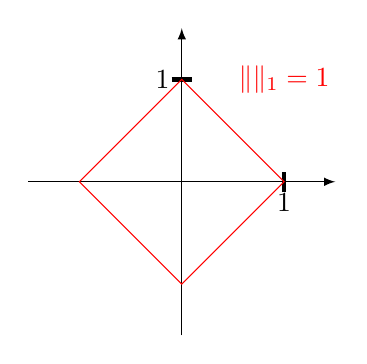
\begin{tikzpicture}[scale=1.3]
    \draw[-latex] (-1.5,0) -- (1.5,0);
    \draw[-latex] (0,-1.5) -- (0,1.5);
    \draw[ultra thick] (1,-0.1) -- (1,0.1) node[below=4pt]{$1$};
    \draw[ultra thick] (-0.1,1) -- (0.1,1) node[left=4pt]{$1$};
    \draw[red] (1,0) -- (0,1) -- (-1,0) -- (0, -1) -- cycle;
    \node[red] at (1,1) {$\|\x\|_1 = 1$};
\end{tikzpicture}
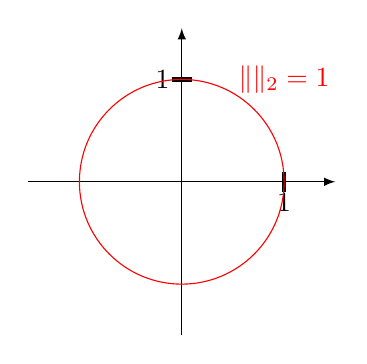
\begin{tikzpicture}[scale=1.3]
    \draw[-latex] (-1.5,0) -- (1.5,0);
    \draw[-latex] (0,-1.5) -- (0,1.5);
    \draw[ultra thick] (1,-0.1) -- (1,0.1) node[below=4pt]{$1$};
    \draw[ultra thick] (-0.1,1) -- (0.1,1) node[left=4pt]{$1$};
    \draw[red] (0,0) circle [radius=1];
    \node[red] at (1,1) {$\|\x\|_2 = 1$};
\end{tikzpicture}
\caption{对于不同范数, 红线指示出范数1的向量集.左:曼哈顿范数;右:欧几里德范数}
\end{figure}

\begin{example}[欧几里德范数]
    $\x \in \R^n$的欧几里德范数被定义为
    \begin{equation}
        \|\x\|_2 := \sqrt{\sum^n_{i=1}x^2_i} = \sqrt{\x^\top\x}
    \end{equation}
    它计算$\x$与原点的欧几里得距离。
    图 3.3 的右侧显示了 $\|\x\|_2 = 1$的所有向量$\x \in \R^2$。
    欧几里得范数也称为$\ell_2$范数。
\end{example}
\begin{remark}
    在本书中,如果没有特别说明,我们将默认使用欧几里得范数 (3.4)。
\end{remark}

\section{内积}

内积允许引入直观的几何概念,例如向量的长度和两个向量之间的角度或距离。
内积的一个主要目的是确定向量是否相互正交(orthogonal)。

\subsection{点积}
我们可能已经熟悉一种特定类型的内积,
即$\R^n$中的标量积/点积(scalar/dot product),
它由下式给出
\begin{equation}
    \x^\top \y = \sum^n_{i=1}x_iy_i.
\end{equation}
在本书中,我们将这种特殊的内积称为点积。
然而,内积是具有特定属性的更一般的概念,我们现在将介绍。

\subsection{通用内积}
回忆 2.7 节中的线性映射,我们可以重新排列关于加法和标量乘法的映射。
双线性映射(bilinear mapping)$\Omega$是具有两个参数的映射,它在每个参数中都是线性的,
即,当我们查看一个向量空间$V$
那么对于所有$\x,\y,\z \in V, \lambda, \psi \in \R$有下式成立
\begin{align}
    \Omega(\lambda\x + \psi\y,\z) = \lambda\Omega(\x,\z) + \psi\Omega(\y,\z) \\
    \Omega(\x,\lambda\y + \psi\z) = \lambda\Omega(\x,\y) + \psi\Omega(\x,\z)
\end{align}
这里,(3.6) 断言$\Omega$在第一个参数中是线性的,
而 (3.7) 断言$\Omega$在第二个参数中是线性的(另见(2.87))。
\begin{definition}
    设$V$是一个向量空间,
    $\Omega : V \times V \rightarrow \R$是一个双线性映射,
    它将两个向量映射到一个实数上。那么
    \begin{itemize}
        \item $\Omega$称为对称的,
              如果$\Omega(\x,\y) = \Omega(\y,\x), \forall \x,\y \in V$
              即, 参数的顺序无关紧要.
        \item $\Omega$称为正定的(positive definite), 如果
        \begin{equation}
            \forall \x \in V\backslash\{\0\}:\Omega(\x,\x) > 0,
            \quad \Omega(\0,\0) = 0.
        \end{equation}
    \end{itemize}
\end{definition}
\begin{definition}
    设$V$是一个向量空间,
    $\Omega : V \times V \rightarrow \R$是一个双线性映射,
    它将两个向量映射到一个实数上。那么
    \begin{itemize}
        \item 一个正定的,对称的双线性映射$\Omega:V \times V \rightarrow \R$
              称为$V$的一个内积.我们通常用$\innerproduct{\x}{\y}$代替$\Omega(\x,\y)$
        \item $(V, \innerproduct{\cdot}{\cdot})$称为内积空间或具有内积的(实)向量空间。
              如果我们使用 (3.5) 中定义的点积,我们称$(V, \innerproduct{\cdot}{\cdot})$为欧几里得向量空间。
    \end{itemize}
\end{definition}
我们将在本书中将这些空间称为内积空间
\begin{example}
    考虑$V = \R^2$, 如果我们定义
    \begin{equation}
        \langle\x,\y\rangle := x_1y_1 - (x_1y_2 + x_2y_1) + 2x_2y_2
    \end{equation}
    那么$\langle\cdot,\cdot\rangle$是一个内积但与点积不同.证明留作练习.
\end{example}

\subsection{对称正定矩阵}
对称正定矩阵(symmetric, positive difinite matrices)
在机器学习中起着重要作用,它们是通过内积定义的。
在 4.3 节中,我们将在矩阵分解的上下文中回到对称正定矩阵。
对称正半定矩阵的思想是核(kernels)定义的关键(第 12.4 节)。

考虑一个$n$-维向量空间$V$,
具有内积$\langle\cdot,\cdot\rangle:V \times V \rightarrow \R$(见定义 3.3),
$V$的有序基为$B = (\b_1,\cdots, \b_n)$ 。
回忆第 2.6.1 节,任何向量$\x, \y \in V$都可以写成基向量的线性组合
使得$\x = \sum^n_{i=1}\psi_i\b_i \in V$
和$\y = \sum^n_{j=1}\lambda_j\b_j \in V$, $\psi_i,\lambda_i \in \R$.
由于内积的双线性,下式对所有$\x,\y \in V$成立
\begin{equation}
    \innerproduct{\x}{\y} =
    \left\langle
    \sum^n_{i=1}\psi_i\b_i,
    \sum^n_{j=1}\lambda_j\b_j,
    \right\rangle =
    \sum^n_{i=1}\sum^n_{j=1}\psi_i\langle\b_i,\b_j\rangle\lambda_j =
    \hat{\x}^\top \A \hat{\y},
\end{equation}
其中$A_{ij} := \langle\b_i,\b_j\rangle$,
$\hat{\x},\hat{\y}$是$\x$和$\y$相对于基$B$的坐标。
这意味着内积$\langle\cdot,\cdot\rangle$是通过$\A$唯一确定的。
内积的对称性也表示$\A$是对称的。
此外,内积的正定性(positive difiniteness)意味着
\begin{equation}
    \forall \x \in V\backslash\{\0\}:
    \x^\top \A\x > 0.
\end{equation}
\begin{definition}[对称正定矩阵]
    满足(3.11)的对称矩阵$\A \in \R^{n\times n}$被称为对称正定矩阵或简称正定矩阵。
    如果只有$\geqslant$在(3.11)中成立,那么$\A$被称为对称半正定(symmetric,positive semidefinite)。
\end{definition}

\begin{example}[对称正定矩阵]
     考虑矩阵
     \begin{equation}
         \A_1 =
         \begin{bmatrix}
             9 & 6 \\
             6 & 5
         \end{bmatrix},\quad
         \A_2 =
         \begin{bmatrix}
             9 & 6 \\
             6 & 3
         \end{bmatrix}.
     \end{equation}
\end{example}
$\A_1$是正定的因为它是对称的并且
\begin{subequations}
    \begin{align}
    \x^\top \A_1 \x &=
    \begin{bmatrix}
        x_1 & x_2
    \end{bmatrix}
    \begin{bmatrix}
        9 & 6 \\
        6 & 5
    \end{bmatrix}
    \begin{bmatrix}
        x_1 \\
        x_2
    \end{bmatrix} \\
    &= 9x^2_1 + 12x_1x_2 + 5x^2_2 = (3x_1 + 2x_2)^2 + x^2_2 > 0
    \end{align}
\end{subequations}
对于所有$\x \in V\backslash\{\0\}$成立.
相反, $\A_2$是对称的但是不是正定的,
因为$\x^\top\A_2\x= 9x^2_1 + 12x_1x_2 + 3x^2_2 = (3x_1 + 2x_2)^2 - x^2_2$
可以小于0, 例如$\x = [2,-3]^\top$.

如果$\A \in \R^{n\times n}$是对称正定的, 那么
\begin{equation}
    \langle\x,\y\rangle = \hat{\x}^\top \A \hat{\y}
\end{equation}
定义了相对于有序基$B$的内积, 其中$\hat{\x},\hat{\y}$是$\x,\y \in V$相对于$B$的坐标表示.

\begin{theorem}
    对于实值有限维向量空间$V$和$V$的有序基$B$,
    $\langle\cdot,\cdot\rangle: V \times V \rightarrow \R$是内积
    当且仅当存在对称正定矩阵$\A \in \R^{n\times n}$且
    \begin{equation}
        \langle\x,\y\rangle = \hat{\x}^\top \A \hat{\y}
    \end{equation}
\end{theorem}

如果$\A \in \R^{n\times n}$对称且正定,则以下性质成立:
\begin{itemize}
    \item $\A$的零空间(核)仅由$\0$组成,
           因为对于所有$\x \neq 0$,$\x^\top\A\x > 0$。
           这意味着如果$\x \neq \0$,则$\A\x \neq 0$。
    \item $\A$的对角元素$a_{ii}$为正,
          因为$a_{ii} = \e_i^\top\A\e_i > 0$,
          其中$\e_i$是$\R^n$中标准基的第$i$个向量。
\end{itemize}

\section{长度和距离}
在 3.1 节中,我们已经讨论了可以用来计算向量长度的范数。
内积和范数密切相关,因为任何内积都会自然而然的产生范数
\begin{equation}
    \|\x\| := \sqrt{\langle\x,\x\rangle}
\end{equation}
这样我们就可以使用内积计算向量的长度。
然而,并不是每个范数都是由内积产生的。
曼哈顿范数 (3.3) 就是一例,它是没有相应内积的范数。
下面,我们将重点介绍由内积导出的范数,并介绍一些几何概念,例如长度、距离和角度。
\begin{remark}[Cauchy-Schwarz不等式]
    对于内积向量空间$(V, \langle\cdot,\cdot\rangle)$,
    范数$\|\cdot\|$满足Cauchy-Schwarz不等式
    \begin{equation}
        |\langle\x,\y\rangle| \leqslant \|\x\|\|\y\|.
    \end{equation}
    \hfill $\lozenge$
\end{remark}

\begin{example}[使用内积的向量长度]
    在几何中,我们经常对向量的长度感兴趣。我们现在可以通过(3.16)来计算内积。
    让我们取$\x = [1, 1]^\top \in \R^2$。
    如果我们使用点积作为内积,用(3.16)我们得到
    \begin{equation}
        \|\x\| = \sqrt{\x^\top\x} = \sqrt{1^2 + 1^2} = \sqrt{2}
    \end{equation}
    作为$\x$的长度.现在让我们选择一个不同的内积:
    \begin{equation}
        \innerproduct{\x}{\y} :=
        \x^\top
        \begin{bmatrix}
            1 & -\frac{1}{2} \\
            -\frac{1}{2} & 1
        \end{bmatrix}
        \y =
        x_1y_1 - \frac{1}{2}(x_1y_2 + x_2y_1) + x_2y_2.
    \end{equation}
    如果我们计算向量的范数,
    那么如果$x_1$和$x_2$具有相同的符号(并且$x_1x_2 > 0$),
    则该内积返回的值小于点积;
    否则,它返回比点积更大的值。
    有了这个内积,我们得到
    \begin{equation}
        \innerproduct{\x}{\x} =
        x_1^2 - x_1x_2 + x_2^2 = 1 - 1 + 1 = 1 \Rightarrow \|\x\| = \sqrt{1} = 1,
    \end{equation}
    这样$\x$的内积的比点积的“短”。
\end{example}

\begin{definition}[距离和距离函数]
    考虑内积空间$(V,\innerproduct{\cdot}{\cdot})$.那么
    \begin{equation}
        d(\x,\y) := \|\x-\y\| = \sqrt{\innerproduct{\x-\y}{\x-\y}}
    \end{equation}
    称为$\x,\y$间的距离,$\x,\y \in V$.
    如果我们使用点积作为内积, 那么这个距离称为欧几里德距离.
    映射
    \begin{align}
        d:V \times V &\rightarrow \R \\
        (\x,\y) &\mapsto d(\x,\y)
    \end{align}
    称为距离函数(metric)
\end{definition}

\begin{remark}
    类似于向量的长度,向量之间的距离不需要内积:一个范数就足够了。
    如果我们有一个由内积产生的范数,距离可能会根据内积的选择而变化
    \hfill $\lozenge$
\end{remark}

距离函数$d$满足
\begin{itemize}
    \item $d$是正定的,i.e.,对于所有$\x,\y \in V, d(\x,\y) \geqslant 0$
          且$d(\x,\y) = 0 \Leftrightarrow \x = \y$.
    \item $d$是对称的,i.e., 对于所有$\x,\y \in V, d(\x,\y) = d(\y,\x)$
    \item 三角不等式: 对于所有$\x,\y,\z \in V, d(\x,\z) \leqslant d(x,y) + d(\y,\z)$
\end{itemize}

\begin{remark}
    乍一看,内积和距离函数的属性列表看起来非常相似。
    然而,通过将定义 3.3 与定义 3.6 进行比较,
    我们观察到$\innerproduct{\x}{\y}$和$d(\x, \y)$行为相反。
    非常相似的$\x$和$\y$将导致内积的大值和距离函数的小值
    \hfill $\lozenge$
\end{remark}

\section{角和正交}
除了能够定义向量的长度以及两个向量之间的距离之外,
内积还通过定义两个向量之间的角度$\omega$来获取向量空间的几何形状。
我们使用 Cauchy-Schwarz 不等式 (3.17)
来定义两个向量$\x, \y$之间的内积空间中的角度$\omega$,
这个概念与恰巧与我们在$\R_2$和$R_3$中的直觉一致。
假设$\x \neq 0, \y \neq 0$. 然后
\begin{equation}
    -1 \leqslant
    \frac{\innerproduct{\x}{\y}}{\|\x\|\|\y\|}
    \leqslant 1.
\end{equation}
因此, 存在唯一的$\omega \in [0,\pi]$, 如图 3.4 所示,有
\begin{equation}
    \cos \omega = \frac{\innerproduct{\x}{\y}}{\|\x\|\|\y\|}
\end{equation}

\begin{figure}
    \begin{tikzpicture}
        \begin{axis}[xlabel=$\omega$, ylabel=$\cos(\omega)$, domain=0:pi]
            \addplot[color=blue,samples=1000] {cos(x)};
        \end{axis}
    \end{tikzpicture}
    \caption{
        当限制为$[0, \pi]$时,
        $f(\omega) = \cos(\omega)$返回区间$[−1, 1]$中的唯一数字。
    }
\end{figure}
数字$\omega$是向量$\x$和$\y$之间的角度。
直观地说,两个向量之间的角度告诉我们它们的方向有多相似。
例如,使用点积,$\x$和$\y = 4\x$之间的角度,
即$\y$是$\x$的缩放版本,为$0$:它们的方向相同。

\begin{example}[向量夹角]
    让我们计算向量$\x = [1,1]^\top \in \R^2,\y = [1,2]^\top \in \R^2$间的角;
    参考图3.5, 我们使用点积作为内积.然后我们有
    \begin{equation}
        \cos \omega =
        \frac{\innerproduct{\x}{\y}}{\sqrt{\innerproduct{\x}{\x},\innerproduct{\y}{\y}}}
        = \frac{\x^\top \y}{\sqrt{\x^\top\x \y^\top\y}}
        = \frac{3}{\sqrt{10}}
    \end{equation}
    所以两个向量间的角度为$\arccos(\frac{3}{\sqrt{10}}) \approx 0.32$rad,
    这大约是$18^\circ$
\end{example}

内积的一个关键特性是它还允许我们表征正交的向量。
\begin{definition}[正交]
    两个向量$\x$和$\y$是正交的(orthogonal),当且仅当$\innerproduct{\x}{\y}= 0$,我们写成$\x \perp \y$。
    如果另外$\|\x\| = 1 = \|\y\|$,即向量是单位向量,则$\x$和$\y$是正交的。
\end{definition}
这个定义的一个含义是$\0$-向量与向量空间中的每个向量都是正交的。
\begin{remark}
    正交将垂直概念推广到不必是点积的双线性形式(bilinear forms)。
    在我们的上下文中,几何上,我们可以将正交向量视为相对于特定内积具有直角(right angle)。
    \hfill $\lozenge$
\end{remark}

\begin{figure}
    \begin{tikzpicture}[-latex]
        \draw[-latex] (-0.01,0) -- (1.5,0);
        \draw[-latex] (0, -0.01) -- (0,2.5);
    \end{tikzpicture}
    \caption{两个向量$\x, \y$之间的角度$\omega$使用内积计算。}
\end{figure}
\begin{example}[正交向量]
    考虑两个向量$\x = [1,1]^\top,\y = [-1,1]^\top \in \R^2$;参考图3.6.
    我们有兴趣使用两个不同的内积来确定它们之间的角度$\omega$。
    使用点积作为内积会产生$\x$和$\y$之间的角度$\omega$为$90^\circ$ ,
    使得$\x \perp \y$。
    但是,如果我们选择内积
    \begin{equation}
        \innerproduct{\x}{\y} = \x^\top
        \begin{bmatrix}
            2 & 0 \\
            0 & 1
        \end{bmatrix}
        \y,
    \end{equation}
    我们得到角$\omega$为
    \begin{equation}
        \cos \omega =
        \frac{\innerproduct{\x}{\y}}{\|\x\|\|\y\|} =
        -\frac{1}{3}
        \Rightarrow \omega \approx 1.91 rad \approx 109.5^\circ,
    \end{equation}
    并且$\x$和$\y$不正交。
    因此,相对于一个内积正交的向量不必相对于不同的内积正交。
\end{example}

\begin{definition}[正交矩阵]
    方阵$\A \in \R^{n\times n}$是正交矩阵, 当且仅当它的列正交(orthonormal)使得
    \begin{equation}
        \A\A^\top = \I = \A^\top\A,
    \end{equation}
    这意味着
    \begin{equation}
        \A^{-1} = \A^\top,
    \end{equation}
    即, 逆矩阵可以简单的通过转置矩阵得到.
\end{definition}

正交矩阵的变换是特殊的,因为向量$\x$的长度在使用正交矩阵$\A$变换时没有改变。
对于点积,我们得到
\begin{equation}
    \|\A\x\|^2 = (\A\x)^\top(\A\x) = \x^\top \A^\top \A\x
    = \x^\top \I \x = \x^\top\x = \|\x\|^2.
\end{equation}
此外,任何两个向量$\x, \y$之间的角度,用它们的内积衡量,
在使用正交矩阵$\A$对它们进行变换时也保持不变。
假设点积作为内积,像$\A\x$和$\A\y$的角度给出为
\begin{equation}
    \cos \omega =
    \frac{(\A\x)^\top(\A\y)}{\|\A\x\|\|\A\y\|} =
    \frac{\x^\top\A^\top\A\y}{\sqrt{\x^\top\A^\top\A\x\y^\top\A^\top\A\y}} =
    \frac{\x^\top\y}{\|\x\|\|\y\|},
\end{equation}
它给出了$\x$和$\y$之间的角度。
这意味着具有$\A^\top = \A^{−1}$的正交矩阵$\A$保留角度和距离。
事实证明,正交矩阵定义了旋转(rotations)的变换(有翻转(flips)的可能性)。
在 3.9 节中,我们将讨论更多关于旋转的细节。

\section{正交基}
在 2.6.1 节中,我们描述了基向量的性质,
发现在一个$n$-维向量空间中,我们需要$n$-个基向量,即$n$-个线性无关的向量。
在 3.3 和 3.4 节中,我们使用内积来计算向量的长度和向量之间的角度。
在下文中,我们将讨论基向量彼此正交且每个基向量的长度为$1$的特殊情况。
我们将称该基为正交基(orthonormal basis)。

让我们更正式地介绍一下。
\begin{definition}[正交基]
    考虑$n$-维向量空间$V$和$V$的有序基$\{\b_1,\cdots,\b_n\}$,如果
    \begin{align}
        \innerproduct{\b_i}{\b_j} &= 0 \quad \text{对于} i \neq j \\
        \innerproduct{\b_i}{\b_i} &= 1
    \end{align}
\end{definition}
对于所有$i, j = 1,\cdots, n$那么这个基称为标准正交基(ONB,orthonormal basis)。
如果仅满足(3.33),则该基称为正交基。
请注意,(3.34)意味着每个基向量的长度/范数为$1$。

回忆一下 2.6.1 节,我们可以使用高斯消元法来为由一组向量张成的向量空间找到一个基。
假设我们有一个集合$\{\tilde{\b}_1,\cdots, \tilde{\b}_n\}$
是非正交(non-orthogonal)和非规范化(unnormalized)的基向量。
我们将它们连接成一个矩阵$\tilde{\B} = [\tilde{\b}_1,\cdots,\tilde{\b}_n]$
并将高斯消元应用于增广矩阵(第 2.3.2 节)
$[\tilde{\B} \tilde{\B}^\top |\tilde{\B}]$
以获得正交基。
这种迭代构建正交基
$\{\tilde{\b}_1,\cdots,\tilde{\b}_n\}$
称为 Gram-Schmidt 过程 (Strang, 2003)

\begin{example}[正交基]
    欧几里得向量空间$\R^n$的规范/标准基是正交基,其中内积是向量的点积。

    $\R^2$中, 向量
    \begin{equation}
        \b_1 = \frac{1}{\sqrt{2}}
        \begin{bmatrix}
            1 \\ 1
        \end{bmatrix},
        \quad
        \b_2 = \frac{1}{\sqrt{2}}
        \begin{bmatrix}
            1 \\ -1
        \end{bmatrix},
    \end{equation}
    形成正交基, 因为$\b_1^\top\b_2 = 0$且$\|\b_1\| = 1 = \|\b_2\|$.
\end{example}

在第12章和第10章讨论支持向量机和主成分分析时,我们将利用正交基的概念。

\section{正交补}
定义了正交后,我们现在将研究相互正交的向量空间。
当我们从几何视角讨论线性降维(linear dimensionality reduction)时,
这将在第10章中发挥重要作用。

考虑一个$D$-维向量空间$V$和一个$M$-维子空间$U \subseteq V$。
那么它的正交补(orthogonal complement)$U^\perp$是$V$的$(D-M)$-维子空间,
并且包含$V$中所有的,与$U$的每个向量都正交的向量。
此外,$U \bigcap U^\perp = \{\0\}$使得任何向量$\x \in V$都可以唯一地分解为
\begin{equation}
    \x = \sum_{m=1}^{M}\lambda_m\b_m
    + \sum_{j=1}^{D-M}\psi_j\b_j^\perp,\quad
    \lambda_m,\psi_j \in \R,
\end{equation}
其中$(\b_1,\cdots,\b_M)$是$U$的一个基,
$(\b_1^\perp,\cdots,\b_{D-M}^\perp)$是$U^\perp$的一个基

因此,正交补也可以用来描述三维向量空间中的平面$U$(二维子空间)。
更具体地说,
与平面$U$正交的向量$\bs{w}$是($\|\bs{w}\| = 1$)$U^\perp$的基向量。
图3.7说明了此设置。
所有与$\bs{w}$正交的向量必须(通过构造)位于平面$U$中。
向量$w$称为$U$的法向量(normal vector)。

通常,正交补可用于描述$n$维向量和仿射空间中的超平面。

\section{函数的内积}
到目前为止,我们研究了内积的属性来计算长度、角度和距离。
我们专注于有限维向量的内积。
下面,我们将看一个不同类型向量的内积示例:函数的内积(inner products of functions)。

到目前为止,我们讨论的内积是为条目数有限的向量定义的。
我们可以将向量$\x \in \R^n$视为具有$n$个函数值的函数。
内积的概念可以推广到具有无限项(可数无限,countably infinite)
和连续值(continuous-valued)函数(不可数无限,uncountably infinite)的向量。
然后向量的各个分量的总和(参见方程(3.5),以此为例)变成一个积分(integral)。

两个函数$u:\R \rightarrow \R$和$v:\R \rightarrow \R$的内积
可以定义为定积分(definite integral)
\begin{equation}
    \innerproduct{u}{v} := \int_a^b u(x)v(x)dx
\end{equation}
下限和上限分别为$a,b < \infty$。
与我们通常的内积一样,我们可以通过查看内积来定义范数和正交。
如果 (3.37) 的计算结果为$0$,则函数$u$和$v$是正交的。
为了使前面的内积在数学上精确,
我们需要注意测度 (measure) 和积分的定义,
从而得到希尔伯特空间(Hilbert space)的定义。
此外,与有限维向量上的内积不同,函数上的内积可能会发散(具有无限值(infinite value))。
所有这一切都需要实函数分析(read and functional analysis)的一些更复杂的细节,我们在本书中没有涉及。

\begin{example}[函数的内积]
    如果我们选择$u = \sin(x)$和$v = \cos(x)$,
    则 (3.37) 的被积函数(integrand)$f(x) = u(x)v(x)$如图 3.8 所示。
    我们看到这个函数是奇函数(odd),即$f(−x) = −f (x)$。
    因此,该乘积的范围为$a = −\pi, b = \pi$的积分为$0$。
    因此,$\sin$和$\cos$是正交函数(orthogonal functions)。
\end{example}
\begin{remark}
    函数的集合
    \begin{equation}
        \{1,\cos(x),\cos(2x),\cos(3x),\cdots\}
    \end{equation}
    是正交的, 如果我们从$-\pi$到$\pi$积分,i.e,
    任何一对函数都是相互正交的。
    (3.38) 中的函数集合张成了一个函数们的巨大的子空间,
    是$[−\pi, \pi)$上的偶函数(even)和周期函数(periodic),
    将函数投影到这个子空间是傅立叶级数(Fourier series)背后的基本思想。
    \hfill $\lozenge$
\end{remark}

在 6.4.6 节中,我们将看看第二种非常规内积:随机变量的内积。

\section{正交投影}
投影是一类重要的线性变换(除了旋转和反射),在图形、编码理论、统计学和机器学习中发挥着重要作用。
在机器学习中,我们经常处理高维数据。
高维数据通常很难分析或可视化。
然而,高维数据往往具有这样的特性,即只有少数维度包含了大部分信息,
而大多数其他维度对于描述数据的关键属性并不是必不可少的。
当我们压缩或可视化高维数据时,我们会丢失信息。
为了最大限度地减少这种压缩损失,我们最好在数据中找到信息量最大的维度。
正如第1章所讨论的,数据可以表示为向量,
在本章中,我们将讨论一些用于数据压缩的基本工具。
更具体地说,我们可以将原始高维数据投影到低维特征空间(feature space),
并在这个低维空间中工作,以了解有关数据集的更多信息并提取相关模式。
例如,机器学习算法,
像Pearson (1901) 和 Hotelling (1933) 的主成分分析 (PCA)
和深度神经网络(deep neural netwrods)(例如,深度自动编码器(Deng 等,2010)),
大量利用了降维的思想。
在下面的,我们将专注于正交投影(orthogonal projections),
我们将在第10章将其用于线性降维,在第12章用于分类。
即使是我们在第 9 章中讨论的线性回归,也可以使用正交投影来解释。
对于给定的低维子空间,高维数据的正交投影保留尽可能多的信息,
并最小化原始数据与相应投影之间的差异(difference)/误差(error)。
图3.9给出了这种正交投影的说明。
在我们详细说明如何获得这些投影之前,让我们先定义投影实际上是什么。

\begin{definition}[投影]
    令$V$为向量空间, 且$U \subseteq V$是$V$的子空间.
    线性映射$\pi : V \rightarrow U$称为投影(projection)如果
    $\pi^2 = \pi \circ \pi = \pi$.
\end{definition}

由于线性映射可以用变换矩阵表示(参见第 2.7 节),
前面的定义同样适用于一种特殊的变换矩阵,
即投影矩阵$\bs{P}_\pi$,它表现出$\bs{P}_\pi^2 = \bs{P}_\pi$的性质。

下面,我们将推导(derive)出
内积空间$(\R^n ,\innerproduct{\cdot}{\cdot})$中向量在子空间上的正交投影。
我们将从一维子空间开始,也称为线(lines)。
如果没有另外提及,我们假设点积$\innerproduct{\x}{\y} = \x^\top \y$作为内积。

\subsection{投影到一维子空间(线)}
假设我们得到一条通过原点的线(一维子空间),
基向量$\b \in \R^n$。
这条线是一个由$\b$张成的一维子空间$U \subseteq \R^n$。
当我们将$\x \in \R^n$投影到$U$上时,
我们寻找最接近$\x$的向量$\pi_U(\x) \in U$。
使用几何参数,让我们描述投影$\pi_U(\x)$的一些属性
(图 3.10(a)作为说明):
\begin{itemize}
    \item 投影$\pi_U(\x)$最接近$\x$,
          其中“最近”意味着距离$\|\x − \pi_U (\x)\|$最小。
          因此,从$\pi_U(\x)$到$\x$的线段$\pi_U(\x) - \x$与$U$正交,
          也就是与$U$的基向量$\b$正交。
          正交条件产生$\innerproduct{\pi_U (\x) − \x}{\b} = 0$,
          因为向量之间的角度是通过内积定义的。
    \item $\x$在$U$上的投影$\pi_U(\x)$必须是$U$的一个元素,
          因此是张成$U$的基向量$\b$的倍数。
          因此,对于某些$\lambda \in R, \pi_U(\x) = \lambda \b$。
\end{itemize}
在以下三个步骤中,我们确定坐标$\lambda$、
投影$\pi_U(\x) \in U$,以及将任意$\x \in \R^n$映射到$U$的投影矩阵$\bs{P}_\pi$:
\begin{enumerate}
    \item 找到坐标$\lambda$。 正交条件产生
    \begin{equation}
        \innerproduct{\x - \pi_U(\x)}{\b} = 0
        \overset{\pi_U(\x)=\lambda\b}{\Longleftrightarrow}
        \innerproduct{\x - \lambda\b}{\b} = 0.
    \end{equation}
    我们现在可以利用内积的双线性并得出
    \begin{equation}
        \innerproduct{\x}{\b} - \lambda\innerproduct{\b}{\b} = 0
        \Longleftrightarrow
        \lambda = \frac{\innerproduct{\x}{\b}}{\innerproduct{\b}{\b}}
        = \frac{\innerproduct{\b}{\x}}{\|\b\|^2}.
    \end{equation}
    在最后一步中,我们利用了内积对称的事实。
    如果我们选择$\innerproduct{\cdot}{\cdot}$作为点积,我们得到
    \begin{equation}
        \lambda =
        \frac{\b^\top\x}{\b^\top\b} =
        \frac{\b^\top\x}{\|\b\|^2}.
    \end{equation}
    如果$\|\b\|=1$, 那么投影的坐标$\lambda$由$\b^\top \x$给出.
    \item 找到投影点$\pi_U(\x) \in U$。
          由于$\pi_U(\x) = \lambda\b$,我们立即用 (3.40) 得到
          \begin{equation}
              \pi_U(\x) = \lambda\b =
              \frac{\innerproduct{\x}{\b}}{\|\b\|^2}\b =
              \frac{\b^\top\x}{\|\b\|^2}\b,
          \end{equation}
          其中最后一个等式仅适用于点积。
          我们还可以通过定义 3.1 计算$\pi_U(\x)$的长度为
          \begin{equation}
              \|\pi_U(\x)\| = \|\lambda\b\| = |\lambda|\|\b\|.
          \end{equation}
          因此,我们的投影长度为$|\lambda|$乘以$\b$的长度。
          这也增加了直觉,即$\lambda$是$\pi_U(\x)$相对于张成我们的一维子空间$U$的基向量$\b$的坐标。

          如果我们使用点积作为内积, 我们有
          \begin{equation}
              \norm{\pi_U(\x)}
              \overset{3.42}{=}
              \frac{|\b^\top\x|}{\norm{\b}^2}\norm{\b}
              \overset{3.25}{=}
              |\cos \omega|
              \norm{\x} \norm{\b}
              \frac{\norm{\b}}{\norm{\b}^2} =
              |\cos \omega|\norm{\x}.
          \end{equation}
          这里,$\omega$是$x$和$b$之间的角度。
          这个方程在三角学中应该很熟悉:
          如果$\|\x\| = 1$,则$\x$位于单位圆上。
          由此可知,$\b$所张成的水平轴上的投影恰好是$\cos \omega$,
          对应向量的长度$\pi_U (\x) = |\cos \omega|$。
          图 3.10(b) 给出了说明。
    \item 找到投影矩阵$\bs{P}_\pi$。
          我们知道投影是线性映射(见定义 3.10)。
          因此,存在一个投影矩阵$\bs{P}_\pi$,
          使得$\pi_U(\x)=\bs{P}_\pi\x$。
          以点积为内积,则
          \begin{equation}
              \pi_U(\x) = \lambda\b = \b\lambda =
              \b \frac{\b^\top\x}{\norm{\b}^2} =
              \frac{\b\b^\top}{\norm{\b}^2}\x,
          \end{equation}
          我们立即看到
          \begin{equation}
              \bs{P}_\pi = \frac{\b\b^\top}{\norm{\b}^2}.
          \end{equation}
          请注意,$\b\b^\top$(因此,$\bs{P}_\pi$)
          是一个对称矩阵(秩为1),
          \footnote{
              译者注: 如果我们有向量$\x$, 我们可以通过$\x\x^\top$来获取一个对称矩阵(超出本人水平不予证明).
              关于对称矩阵秩为1, 超出本人水平不予证明(等我学废了就回来把这俩个坑填了)
          }
          并且$\norm{\b}^2 = \innerproduct{\b}{\b}$是一个标量。
\end{enumerate}
投影矩阵$\bs{P}_\pi$
将任何向量$\x \in \R^n$投影到通过原点且方向为$\b$的直线上
(相当于$\b$张成的子空间$U$)。
\begin{remark}
    投影$\pi_U(\x) \in \R_n$仍然是一个$n$-维向量而不是一个标量。
    然而,我们不再需要$n$个坐标来表示投影,
    如果我们想相对于张成子空间$U: \lambda$的基向量$\b$来表示它,则只需要一个坐标。
    \hfill $\lozenge$
\end{remark}

\begin{example}[投影到一条线上]
    求投影矩阵$\bs{P}_\pi$,它投影到通过原点由$\b = \begin{bmatrix}1 & 2 & 2 \end{bmatrix}^\top$张成的直线上。
    $\b$是一维子空间(通过原点的线)的方向和基。

    使用(3.46),我们得到
    \begin{equation}
        \bs{P}_\pi = \frac{\b\b^\top}{\b^\top\b} =
        \frac{1}{9}
        \begin{bmatrix}
            1 \\ 2 \\ 2
        \end{bmatrix}
        \begin{bmatrix}
            1 & 2 & 2
        \end{bmatrix} =
        \frac{1}{9}
        \begin{bmatrix}
            1 & 2 & 2 \\
            2 & 4 & 4 \\
            2 & 4 & 4
        \end{bmatrix}.
    \end{equation}
    现在让我们选择一个特定的$\x$,看看它是否位于$\b$张成的子空间中。
    对于$\x = \begin{bmatrix} 1 & 1 & 1 \end{bmatrix}^\top$,投影为
    \begin{equation}
        \pi_U(\x) = \bs{P}_\pi\x =
        \frac{1}{9}
        \begin{bmatrix}
            1 & 2 & 2 \\
            2 & 4 & 4 \\
            2 & 4 & 4
        \end{bmatrix}
        \begin{bmatrix}
            1 \\ 1 \\ 1
        \end{bmatrix} =
        \frac{1}{9}
        \begin{bmatrix}
            5 \\ 10 \\ 10
        \end{bmatrix}
        \in \spn[\begin{bmatrix}
            1 \\ 2 \\ 3
        \end{bmatrix}].
    \end{equation}
    请注意,将$\bs{P}_\pi$应用于$\pi_U (\x)$不会改变任何内容,
    即$\bs{P}_\pi \pi_U(\x) = \pi_U(\x)$。
    这是预料之中的,因为根据定义 3.10,
    我们知道投影矩阵$\bs{P}_\pi$对于所有$\x$
    都满足$\bs{P}^2_\pi \x = \bs{P}_ \pi \x$.
\end{example}
\begin{remark}
    根据第4章的结果,我们可以证明$\pi_U(\x)$是$\bs{P}_\pi$的特征向量(eigenvector),对应的特征值(eigenvalue)为 1。
    \hfill $\lozenge$
\end{remark}

\subsection{投影到一般子空间}
下面,我们看看向量$\x \in \R^n$到低维子空间$U \subseteq \R^n$的正交投影,
其中$\dim(U) = m \geqslant 1$。图 3.11 给出了一个说明。

假设$(\b_1,\cdots,\b_m)$是$U$的有序基。
任何在$U$上的投影$\pi_U(\x)$必然是$U$的一个元素。
因此,它们可以表示为$U$的基向量$\b_1,\cdots,\b_m$的线性组合。
使得$\pi_U(\x) = \sum_{i=1}^{m}\lambda_i\b_i$。

与一维情况一样,我们遵循三步程序来找到投影$\pi_U(\x)$和投影矩阵$\bs{P}_\pi$:
\begin{enumerate}
\item 找到投影的坐标$\lambda_1,\cdots,\lambda_m$(相对于$U$的基),使得线性组合
    \begin{align}
        &\pi_U(\x) = \sum_{i=1}^{m}\lambda_i\b_i = \B\bs{\lambda},\\
        &\B = [\b_1,\cdots,\b_m] \in \R^{n\times m},
        \quad
        \bs{\lambda} = [\lambda_1,\cdots,\lambda_m]^\top \in \R^m,
    \end{align}
    最接近$\x \in \R^n$。
    与一维情况一样,“最近”意味着“最小距离”,
    这意味着连接$\pi_U (\x) \in U$和$\x \in \R^n$的向量必须与$U$的所有基向量正交。
    因此,我们得到$m$个同时条件(假设点积为内积)
    \begin{align}
        \innerproduct{\b_1}{\x - \pi_U(\x)} =& \b_1^\top(\x - \pi_U(\x)) = 0\\
        &\vdots \notag\\
        \innerproduct{\b_m}{\x - \pi_U(\x)} =& \b_m^\top(\x - \pi_U(\x)) = 0
    \end{align}
    其中,当$\pi_U (\x) = \B\bs{\lambda}$时,可以写成
    \begin{align}
        \b_1^\top(\x& - \B\bs{\lambda}) = 0 \\
        &\vdots \notag\\
        \b_m^\top(\x& - \B\bs{\lambda}) = 0
    \end{align}
    这样我们就可以得到一个齐次的线性方程组
    \begin{align}
        \begin{bmatrix}
            \b_1^\top \\ \vdots \\ \b_m^\top
        \end{bmatrix}
        \begin{bmatrix}
            \x - \B\bs{\lambda}
        \end{bmatrix}
        = \0
        &\Longleftrightarrow
        \B^\top(\x - \B\bs{\lambda}) = \0 \\
        &\Longleftrightarrow
        \B^\top\B\bs{\lambda} = \B^\top\x.
    \end{align}
    最后一个表达式称为正规方程(normal equation)。
    由于$\b_1,\cdots,\b_m$是$U$的基,因此线性无关,
    $\B^\top \B \in \R^{m \times m}$是正规的,可以求逆。
    这使我们能够求解系数(coefficients)/坐标
    \begin{equation}
        \bs{\lambda} = (\B^\top\B)^{-1}\B^\top\x.
    \end{equation}
    矩阵$(\B^\top \B)^{-1}\B^\top$也称为$\B$的伪逆,可以为非方阵$\B$计算。
    它只要求$\B^\top\B$是正定的,如果$\B$满秩就是这种情况。
    在实际应用中(例如,线性回归),
    我们经常在$\B^\top\B$中添加一个“抖动项(jitter term)”$\epsilon\I$,
    以保证增加数值稳定性和正定性。
    这个“岭(ridge)”可以使用贝叶斯推理严格推导出来。
    有关详细信息,请参阅第 9 章。
\item 求投影$\pi_U(\x) \in U$。
      我们已经确定$\pi_U(\x) = \B\bs{\lambda}$。
      因此,利用 (3.57)
      \begin{equation}
          \pi_U(\x) = \B(\B^\top\B)^{-1}\B^\top\x.
      \end{equation}
\item 找到投影矩阵$\bs{P}_ \pi$。
      从(3.58),我们可以立即看出求解$\bs{P}_\pi \x = \pi_U(\x)$的投影矩阵必须是
      \begin{equation}
          \bs{P}_\pi = \B(\B^\top\B)^{-1}\B^\top.
      \end{equation}
\end{enumerate}
\begin{remark}
    投影到一般子空间的解决方案包括1D情况作为特殊情况:
    如果$\dim(U) = 1$,则$\B^\top\B \in \R$是标量,
    并且我们可以将投影矩阵(3.59)
    $\bs{P}_\pi = \B(\B^\top\B)^{−1}\B^\top$
    重写为
    $\bs{P}_\pi = \frac{\B\B^\top}{\B^\top\B}$,
    这正是(3.46)中的投影矩阵。
    \hfill $\lozenge$
\end{remark}

\begin{example}[投影到二维子空间]
    对于子空间$U = \spn[
        \begin{bmatrix} 1 \\ 1 \\ 1 \end{bmatrix}
        \begin{bmatrix} 0 \\ 1 \\ 2 \end{bmatrix}
    ] \subseteq \R^3$
    和$\x = \begin{bmatrix} 6 \\ 0 \\ 0 \end{bmatrix} \in \R^3$,
    根据子空间$U$,投影点$\pi_U(\x)$和投影矩阵$\bs{P}_\pi$
    找到$\x$的坐标$\bs{\lambda}$.

    首先,我们看到$U$的生成集是一个基(线性独立),将$U$的基向量写成矩阵
    $\B = \begin{bmatrix}
        1 & 0 \\
        1 & 1 \\
        1 & 2 \\
    \end{bmatrix}.$

    第二,我们计算矩阵$\B^\top\B$以及$\B^\top\x$
    \begin{equation}
        \B^\top\B =
        \begin{bmatrix}
            1 & 1 & 1 \\
            0 & 1 & 2
        \end{bmatrix}
        \begin{bmatrix}
            1 & 0 \\
            1 & 1 \\
            1 & 2
        \end{bmatrix} =
        \begin{bmatrix}
            3 & 3 \\
            3 & 5
        \end{bmatrix},\quad
        \B^\top\x =
        \begin{bmatrix}
            1 & 1 & 1 \\
            0 & 1 & 2
        \end{bmatrix}
        \begin{bmatrix}
            6 \\ 0 \\ 0
        \end{bmatrix} =
        \begin{bmatrix} 6 \\ 0 \end{bmatrix}.
    \end{equation}

    第三, 我们求解正规方程$\B^\top\B\bs{\lambda}=\B^\top\x$来找到$\bs{\lambda}$:
    \begin{equation}
        \begin{bmatrix}
            3 & 3 \\
            3 & 5
        \end{bmatrix}
        \begin{bmatrix}
            \lambda_1 \\ \lambda_2
        \end{bmatrix} =
        \begin{bmatrix}
            6 \\ 0
        \end{bmatrix}
        \Longleftrightarrow
        \bs{\lambda} =
        \begin{bmatrix}
            5 \\ -3
        \end{bmatrix}.
    \end{equation}

    第四, $\x$在$U$上的投影$\pi_U(\x)$,i.e,进入$\B$的列空间,可以通过直接计算
    \begin{equation}
        \pi_U(\x) = \B\bs{\lambda} = \begin{bmatrix} 5 \\ 2 \\ -1 \end{bmatrix}.
    \end{equation}
    对应的投影误差(projection error)是原始向量与其$U$上投影的差向量(difference vector)的范数,即
    \begin{equation}
        \norm{\x - \pi_U(\x)} =
        \norm{\begin{bmatrix}1 & -2 & 1\end{bmatrix}^\top} = \sqrt{6}.
    \end{equation}

    第五, 投影矩阵(对于任意$\x \in \R^3)$为
    \begin{equation}
        \bs{P}_\pi = \B(\B^\top\B)^\top B^\top =
        \frac{1}{6}
        \begin{bmatrix}
            5 & 2 & -1 \\
            2 & 2 & 2 \\
            -1 & 2 & 5
        \end{bmatrix}.
    \end{equation}
    为了验证结果,我们可以
    (a)检查位移向量$\pi_U(\x) − \x$是否与$U$的所有基向量正交,以及
    (b)验证$\bs{P}_\pi = \bs{P}_\pi^2$(参见定义 3.10)。
\end{example}
\begin{remark}
    尽管投影$\pi_U(\x)$位于$m$-维子空间$U \subseteq \R^n$中,
    但它们仍然是$\R^n$中的向量。
    然而,为了表示一个投影向量,
    我们只需要$m$个坐标$\lambda_1,\cdots, \lambda_m$,
    这相对于$U$的基向量$\b_1,\cdots, \b_m$。
    \hfill $\lozenge$
\end{remark}
\begin{remark}
    在具有一般内积的向量空间中,
    我们在计算角度和距离时要注意,
    它们是由内积定义的。
    \hfill $\lozenge$
\end{remark}

投影允许我们查看线性方程组$\A\x = \b$没有解的情况。
回想一下,这意味着$\b$不在$\A$的张成内,
即向量$\b$不在$\A$的列所张成的子空间中。
鉴于无法精确求解线性方程,我们可以找到一个近似解(approximate solution)。
这个想法是在$\A$的列所张成的子空间中找到与$\b$最接近的向量,
即我们计算$\b$在$\A$列所张成的子空间上的正交投影。
这个问题在实践中经常出现,
并且解称为超定系统(overdeterminded system)的最小二乘解(least-squares solution)
(假设点积为内积)。
这将在第9.4节中进一步讨论。
使用重构误差(reconstruction errors) (3.63) 是推导主成分分析的一种可能方法(第 10.3 节)。

\begin{remark}
    我们只是查看了向量$\x$在子空间$U$上的投影,
    其基向量为${\b_1,\cdots,\b_k}$。
    如果这个基是ONB,即满足(3.33)和(3.34),
    则投影方程(3.58)大大简化为
    \begin{equation}
        \pi_U(\x) = \B\B^\top\x
    \end{equation}
    因为$\B^\top \B = \I$, 坐标
    \begin{equation}
        \bs{\lambda} = \B^\top \x.
    \end{equation}
    这意味着我们不再需要从(3.58)计算逆,这节省了计算时间。
    \hfill $\lozenge$
\end{remark}

\subsection{Gram-Shmidt 正交化}
投影是 Gram-Schmidt 方法的核心,
它允许我们建设性地将$n$-维向量空间$V$的任何基
$(\b_1,\dots,\b_n)$转换为$V$的正交/正交
\footnote{ 原文为 orthogonal/orthonormal, 都翻译为"正交" }
基$(\u_1,\dots,\u_n)$ 。
该基始终存在(Liesen 和 Mehrmann,2015 年)且
$\spn[\b_1,\dots, \b_n ] = \spn[\u_1,\dots ,\u_n]$。
Gram-Schmidt 正交化(orthogonalization)方法
从$V$的任何基$(\b_1,\dots, \b_n)$
迭代地构造正交基$(\u_1,\dots\u_n )$,如下:
\begin{align}
    &\u_1 := \b_1 \\
    &\u_k := \b_k - \pi_{\spn[\u_1,\cdots,\u_{k-1}]}(\b_k),
    \quad
    k = 2,\cdots,n.
\end{align}
在(3.68)中,
第$k$个基向量$\b_k$被投影到由前$k-1$个
被构造的正交向量$\u_1,\dots,\u_{k−1}$
所张成的子空间上;见第 3.8.2 节。
然后从$\b_k$中减去该投影并产生一个向量$\u_k$,
该向量与$\u_1,\dots,\u_{k−1}$张成的$(k − 1)$维子空间正交。
对所有$n$个基向量$\b_1,\dots, \b_n$重复此过程。
产生$V$的正交基$(\u_1,\dots,\u_n)$。
如果我们对$\u_k$进行归一化(normalize),
我们将获得一个 ONB,其中$\norm{\u_k} = 1$,$k = 1,\dots,n$.

\begin{example}[Gram-Schmidt 正交化]
    考虑$\R^2$的基$(\b_1,\b_2)$, 其中
    \begin{equation}
        \b_1 = \begin{bmatrix} 2 \\ 0 \end{bmatrix}
        \quad
        \b_2 = \begin{bmatrix} 1 \\ 1 \end{bmatrix};
    \end{equation}
    另请参见图 3.12(a)。
    使用 Gram-Schmidt 方法,
    我们构造$\R^2$的正交基$(\u_1, \u_2)$如下(假设点积为内积):
    \begin{align}
        &\u_1 := \b_1 = \begin{bmatrix} 2 \\ 0 \end{bmatrix}, \\
        &\u_2 := \b_2 - \pi_{\spn[\u_1]}(\b_2)
        \overset{(3.45)}{=}
        \b_2 - \frac{\u_1\u_1^\top}{\norm{\u_1}^2}\b_2 =
        \begin{bmatrix}
            1 \\ 1
        \end{bmatrix}
        \begin{bmatrix}
            1 & 0 \\
            0 & 0
        \end{bmatrix}
        \begin{bmatrix}
            1 \\ 1
        \end{bmatrix} =
        \begin{bmatrix}
            0 \\ 1
        \end{bmatrix}.
    \end{align}
\end{example}
这些步骤如图 3.12(b) 和 (c) 所示。
我们立即看到$\u_1$和$\u_2$是正交的,
即$\u_1^\top \u_2 = 0$。

\subsection{投影到仿射子空间}
到目前为止,我们讨论了如何将向量投影到低维子空间$U$上。
在下文中,我们提供了将向量投影到仿射子空间的解决方案。

考虑图 3.13(a) 中的设置。
给定一个仿射空间$L = \x_0 + U$,其中$\b_1,\b_2$是$U$的基向量。
为了确定$\x$在$L$上的正交投影$\pi_L(\x)$,
我们将问题转化为一个我们知道如何解决的问题:在向量子空间上的投影。
为此,我们从$\x$和$L$中减去支持点$\x_0$,
这样$L − \x_0 = U$就是向量子空间$U$。
我们现在可以使用我们在 3.8.2 节中讨论的子空间上的正交投影,
并获得投影$\pi_U (\x − \x_0)$,如图 3.13(b) 所示。
现在可以通过添加$\x_0$将该投影转换回$L$ ,
这样我们就可以得到在仿射空间$L$上的正交投影为
\begin{equation}
    \pi_L(\x) = \x_0 + \pi_U(\x - \x_0),
\end{equation}
其中$\pi_U(\cdot)$是子空间$U$上的正交投影,i.e.,$L$的方向空间;参考图3.13(c).

从图 3.13 也可以看出,$\x$到仿射空间$L$的距离等于$\x − \x_0$到$U$的距离, 即,
\begin{subequations}
    \begin{align}
        d(\x,L) =
        \norm{\x - \pi_L(\x)} =
        \norm{\x - (\x_0 + \pi_U(\x - \x_0))} \\
        = d(\x - \x_0, \pi_U(\x - \x_0))
        = d(\x - \x_0, U).
    \end{align}
\end{subequations}

我们将在 12.1 节中使用仿射子空间上的投影来推导出分离超平面(separating hyperplane)的概念。

\section{旋转}
如第 3.4 节所述,长度和角度保持不变,是正交变换矩阵线性映射的两个特征。
在下文中,我们将仔细研究描述旋转的特定正交变换矩阵。

旋转是一种线性映射(更具体地说,是欧几里得向量空间的自同构),
它使平面绕原点旋转角度$\theta$,即原点是一个不动点(fixed point)。
对于正角$\theta > 0$,按照惯例,我们以逆时针方向旋转。
示例如图 3.14 所示,其中变换矩阵为
\begin{equation}
    \bs{R} =
    \begin{bmatrix}
        -0.38 & -0.92 \\
        0.92 & -0.38
    \end{bmatrix}
\end{equation}
旋转的重要应用领域包括计算机图形学(computer graphics)和机器人学(robotics)。
例如,在机器人技术中,了解如何旋转机械臂的关节以拾取或放置物体通常很重要,请参见图 3.15。

\subsection{$\R^2$中的旋转}
考虑$\R^2$标准基
$
\left\{
    \e_1 = \begin{bmatrix} 1 \\ 0 \end{bmatrix},
    \e_2 = \begin{bmatrix} 0 \\ 1 \end{bmatrix}
\right\}
$
这定义了$\R^2$的标准坐标系.
我们的目标是将这个坐标系旋转一个角度$θ$,如图 3.16 所示。
请注意,旋转矢量仍然是线性无关的,因此是$\R^2$的基。
这意味着旋转进行了基变换.

旋转$\Phi$是线性映射,因此我们可以用旋转矩阵$\bs{R}(\theta)$表示它们。
三角学(见图 3.16)允许我们确定旋转轴($\Phi$的像)相对于$\R^2$中的标准基的坐标。
我们有
\begin{equation}
    \Phi(\e_1) =
    \begin{bmatrix}
        \cos \theta \\
        \sin \theta
    \end{bmatrix},
    \Phi(\e_2) =
    \begin{bmatrix}
        - \sin \theta \\
        \cos \theta
    \end{bmatrix}.
\end{equation}
因此,将基变换为旋转坐标$\bs{R}(\theta)$的旋转矩阵为
\begin{equation}
    \bs{R}(\theta) = [\Phi(\e_1), \Phi(\e_2)] =
    \begin{bmatrix}
        \cos \theta & - \sin \theta \\
        \sin \theta & \cos \theta
    \end{bmatrix} .
\end{equation}

\subsection{$\R^3$中的旋转}
与$\R^2$的情况相反,在$\R^3$中,我们可以围绕一维轴旋转任何二维平面。
指定通用旋转矩阵的最简单方法是指定标准基$\e_1、\e_2、\e_3$的像应该如何旋转,
并确保这些像$\bs{R}\e_1、\bs{R}\e_2、\bs{R}\e_3$彼此正交。
然后我们可以通过组合标准基的像来获得一个通用的旋转矩阵$\bs{R}$。

要获得有意义的旋转角度,
我们必须定义在二维以上操作时“逆时针”的含义。
我们使用的约定是,当我们查看“从末端到原点”的轴时,
关于轴的“逆时针”(平面)旋转是指绕轴的旋转。
因此,在$\R_3$中,围绕三个标准基向量进行了三个(平面)旋转(见图 3.17):
\begin{itemize}
    \item 绕$\e_1$-轴旋转
    \begin{equation}
         \bs{R}_1(\theta) =
         [\Phi(\e_1), \Phi(\e_2),\Phi(\e_3)] =
         \begin{bmatrix}
             1 & 0 & 0 \\
             0 & \cos \theta & -\sin \theta \\
             0 & \sin \theta & \cos \theta \\
         \end{bmatrix}.
    \end{equation}
    这里,$\e_1$坐标固定,在$\e_2$$\e_3$平面逆时针旋转。
    \item 绕$\e_2$-轴旋转
    \begin{equation}
        \bs{R}_2(\theta) =
        \begin{bmatrix}
            \cos \theta & 0 & \sin \theta \\
            0 & 1 & 0 \\
            -\sin(\theta) & 0 & \cos \theta
        \end{bmatrix}.
    \end{equation}
    如果我们围绕 $\e_2$ 轴旋转 $\e_1$ $\e_3$ 平面,
    我们需要从 $\e_2$ 轴的“尖端”朝向原点观察。
    \item 绕 $\e_3$ 轴旋转
    \begin{equation}
        \bs{R}^3(\theta) =
        \begin{bmatrix}
            \cos \theta & -\sin \theta & 0 \\
            \sin \theta & \cos \theta & 0 \\
            0 & 0 & 1
        \end{bmatrix}.
    \end{equation}
    图 3.17 说明了这一点。
\end{itemize}

\subsection{在$n$维中旋转}
将旋转从 2D 和 3D 推广到$n$维欧几里得向量空间可以直观地描述为
固定$n - 2$维并将旋转限制在$n$维空间中的二维平面。
在三维情况下,我们可以旋转任何平面($\R^n$的二维子空间)。

\begin{definition}[吉文斯轮换]
    设$V$是一个$n$维欧几里得向量空间
    且$\Phi : V \rightarrow V$是自同构,其具有变换矩阵
    \begin{equation}
        \bs{R}_{ij}(\theta) :=
        \begin{bmatrix}
            \I_{i-1} & \0 & \cdots & \cdots & \0 \\
            \0 & \color{red}\cos \theta & \0 & \color{red}-\sin \theta & \0 \\
            \0 & \0 & \I_{j-i-1} & \0 & \0 \\
            \0 & \color{red}\sin \theta & \0 & \color{red}\cos \theta & \0 \\
            \0 & \cdots & \cdots & \0 & \I_{n-j} \\
        \end{bmatrix}
        \in \R^{n \times n},
    \end{equation}
    其中$1 \leqslant i < j \leqslant n, \theta \in \R$.
    那么$\bs{R}_{ij}(\theta)$称为吉文斯轮换(Givens Rotation).
    本质上,$\bs{R}_{ij}(\theta)$是单位矩阵$\I_n$,其
    \begin{equation}
        r_{ii} = \cos \theta,
        r_{ij} = -\sin \theta,
        r_{ji} = \sin \theta,
        r_{jj} = \cos \theta.
    \end{equation}
    在二维(即 n = 2)中,我们得到 (3.76) 作为特例。
\end{definition}

\subsection{旋转的性质}
旋转表现出许多有用的性质,
可以通过将它们视为正交矩阵(定义 3.8)来推导出这些属性:
\begin{itemize}
    \item 旋转保持距离,即
    $\norm{\x-\y} = \norm{\bs{R}_\theta (\x)−\bs{R}_\theta(\y)}$。
    换句话说,旋转使变换后任意两点之间的距离保持不变。
    \item 旋转保持角度,即
    $\bs{R}_\theta \x$和$\bs{R}_\theta \y$之间的角度等于$\x$和$\y$之间的角度。
    \item 三维(或更多维)的旋转通常不是可交换的。
    因此,应用旋转的顺序很重要,即使它们围绕同一点旋转。
    只有在二维向量旋转是可交换的,使得
    $\bs{R}(\phi)\bs{R}(\theta) = \bs{R}(\theta)\bs{R}(\phi)$
    对于所有$\phi, \theta \in [0, 2\pi)$成立。
    只有当它们围绕同一点(例如原点)旋转时,它们才形成阿贝尔群(有乘法)。
\end{itemize}

\section{深入阅读}
在本章中,我们简要概述了解析几何的一些重要概念,我们将在本书后面的章节中使用这些概念。
对于我们提出的一些概念的更广泛和更深入的概述,我们参考以下优秀书籍:Axler (2015) and Boyd and Vandenberghe (2018)。

内积允许我们使用 Gram-Schmidt 方法确定向量(子)空间的特定基,
其中每个向量与所有其他向量(正交基)正交。
这些基础在求解线性方程组的优化和数值算法中很重要。
例如,Krylov子空间方法,
例如共轭梯度或广义最小残差方法 (GMRES),
可最小化彼此正交的残差误差 (Stoer 和 Burlirsch,2002)。

在机器学习中,内积在核方法的上下文中很重要(Schölkopf 和 Smola,2002)。
核方法利用了许多线性算法可以纯粹通过内积计算来表达的事实。
然后,“核技巧”允许我们在(可能是无限维的)特征空间中隐式计算这些内积,
甚至无需明确知道这个特征空间。
这允许机器学习中使用的许多算法的“非线性化”,
例如用于降维的 kernel-PCA (Schölkopf et al., 1997)。
高斯过程(Rasmussen 和 Williams,2006)也属于核方法的范畴,
并且是概率回归(拟合数据点的曲线)的最新技术。
内核的概念在第 12 章进一步探讨。

投影通常用于计算机图形中,例如,生成阴影。
在优化中,正交投影通常用于(迭代地)最小化残差。
这在机器学习中也有应用,例如,在线性回归中,我们希望找到一个(线性)函数来最小化残差,
即数据在线性函数上的正交投影的长度(Bishop,2006)。
我们将在第 9 章对此进行进一步研究。
PCA(Pearson,1901;Hotelling,1933)还使用投影来降低高维数据的维数。
我们将在第 10 章中更详细地讨论这一点。

\section*{练习题}
